\documentclass[12pt]{article}

%%%%%%%%%%%%%%%%%%%%%%%%%%%%
%%%%%%%%%%%%%%%%%%%%%%%%%%%%
% Load in packages
\usepackage{amsmath}
\usepackage{amssymb}
\usepackage{hyperref}
\usepackage{graphicx}
\usepackage[top=1in, bottom=1in, left=1in, right=1in]{geometry}

%%%%%%%%%%%%%%%%%%%%%%%%%%%%
%%%%%%%%%%%%%%%%%%%%%%%%%%%%

\begin{document}

\begin{center}
\Large Chapter 3 Practice Problems

\medskip

\normalsize Elements of Microeconomics (discussion section 4)

\medskip

\small Jamie Hyder
\end{center}

\medskip

\section*{Question 1}

Muffin's Steakhouse and Sandy's Salads are two restaurants which serve salads and steaks, respectively. Given 1000 minutes of labor time, they can produce the following amounts of each dish:

\begin{table}[h]
  \centering
  \begin{tabular}{|c|c|c|}
    \hline
    \textbf{Restaurant} & \textbf{Steaks} & \textbf{Salads} \\
    \hline
    \textbf{Muffin's Steakhouse} & 100 & 20 \\
    \hline
    \textbf{Sandy's Salads} & 200 & 100 \\
    \hline
  \end{tabular}
  \caption{Muffin vs. Sandy}
\end{table}

\begin{enumerate}

\item What is their cost, in minutes, to produce steak and salads?

\medskip

\textbf{Answer:}

\begin{table}[h]
  \centering
  \begin{tabular}{|c|c|c|}
    \hline
    \textbf{Restaurant} & \textbf{Minutes per steak} & \textbf{Minutes per salad} \\
    \hline
    \textbf{Muffin's Steakhouse} & 10 & 50 \\
    \hline
    \textbf{Sandy's Salads} & 5 & 10 \\
    \hline
  \end{tabular}
  \caption{Muffin vs. Sandy}
\end{table}


\item Assume that there is a \textit{constant transferability} of productive resources from one dish to the other:
\begin{enumerate}
    \item Draw the production possibility frontiers for the two restaurants.
    \item Who has the absolute advantage in producing steaks?
    \item Who has the absolute advantage in producing salads?
\end{enumerate}

\textbf{Answer:}

\textbf{a.} The two PPFs should look like figures \ref{fig:MuffinPPF} and \ref{fig:SandyPPF}.

\begin{figure}
    \centering
    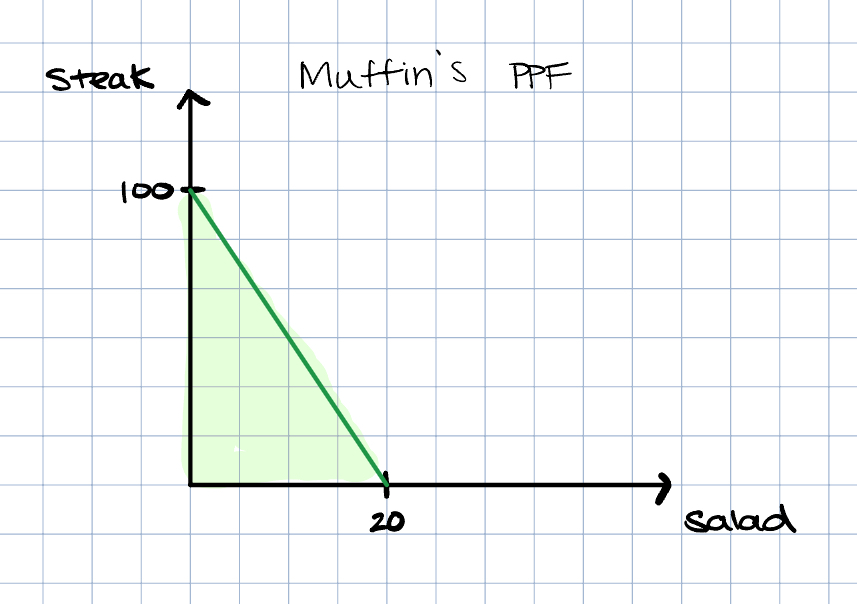
\includegraphics[width=.6\textwidth]{MuffinsPPF.png}
    \caption{PPF of Muffin's Steakhouse}
    \label{fig:MuffinPPF}
\end{figure}

\begin{figure}
    \centering
    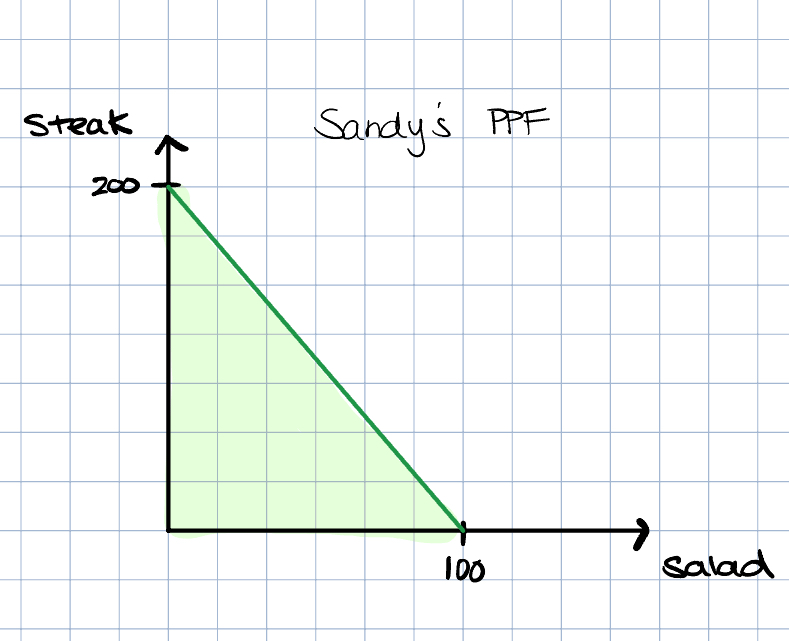
\includegraphics[width=.6\textwidth]{SandysPPF.png}
    \caption{PPF of Sandy's Salads}
    \label{fig:SandyPPF}
\end{figure}

\textbf{b. and c.} Sandy has the absolute advantage in both dishes, since the time that it takes her to produce both steaks and salads is less than the time that it takes Sue to produce the dishes. 

\newpage

\item Let's think about the opportunity cost of each firm for each dish:
\begin{enumerate}
    \item What are the slopes of the two PPFs?
    \item What is Muffin's opportunity cost for producing steaks and salads?
    \item What is Sandy's opportunity cost for producing steaks and salads?
\end{enumerate}

\textbf{Answer:}

\textbf{a.} The slope of Muffin's PPF is $-5$ and the slope of Sandy's PPF is $-2$.
Muffin: \(\frac{-100}{20} = -5\)
Sandy: \(\frac{-200}{100} = -2\)

\textbf{b.} Muffin faces an opportunity cost to produce 1 steak of \[oc = \frac{\Delta salad}{\Delta steak } = \frac{20-0}{100-0} = \frac{20}{100} = \frac{1}{5}\] of a salad. The opportunity cost to produce 1 salad, on the other hand, is 5 steaks (\(oc = \frac{\Delta steak}{\Delta salad } = \frac{100-0}{20-0} = \frac{100}{20} = 5\)). Notice that the opportunity cost of one dish is the inverse of the other. 

\textbf{c.} Sandy faces an opportunity cost to produce 1 steak of \[oc = \frac{\Delta salad}{\Delta steak } = \frac{100-0}{200-0} = \frac{100}{200} =\frac{1}{2}\] of a salad, and the opportunity cost to produce 1 salad of \[oc = \frac{\Delta steak}{\Delta salad} = \frac{200-0}{100-0} = \frac{200}{100} =\frac{2}{1} = 2\] steaks.

\medskip
\medskip
\medskip

\item 
\begin{enumerate}
    \item Can a firm have an absolute advantage in both goods?
    \item Can a firm have a comparative advantage in both goods?
    \item What is the relationship between the comparative advantage in good A and good B?
\end{enumerate}

\textbf{Answer:}

\textbf{a.} Yes; in our example, Sandy has the absolute advantage for both goods.

\medskip

\textbf{b.} No; if one firm has a comparative advantage with one good, that relationship is flipped for the other good.

\medskip

\textbf{c.} They are \textit{inverses}, and this underlies the answer to question 2. This is because of how fractions work, but there is clear intuition: if the opportunity cost for good A is really small, then the opportunity cost for good B must be very large.

\medskip
\medskip
\medskip

\item Since most customers like to order a salad with their steak, Sandy and Muffin both want to offer both salads and steaks (not necessarily in equal quantities since some customers will only want one or the other).

\begin{enumerate}
    \item If both restaurants spend half their resources on each dish, what is their output?
    \item Assume the two businesses can trade. What is one set of productions, and one possible exchange, which would leave them both better off?
\end{enumerate}

\textbf{Answer:}

\textbf{a.} If they divide their 1000 minutes evenly between the two goods their output is given in table \ref{tab:tab3}.

\begin{table}
    \begin{tabular}{|c|c|c|}
      \hline
      \textbf{Restaurant} & \textbf{Steaks} & \textbf{Salads} \\
      \hline
      \textbf{Muffin's Steakhouse} & 50 & 10 \\
      \hline
      \textbf{Sandy's Salads} & 100 & 50 \\
      \hline
      \textbf{Total output} & 150 & 60 \\
      \hline
    \end{tabular}
    \caption{50/50 split}
  \end{table}

\textbf{b.} There are many possible answers here (in fact, an infinite number), and I will only present one.

\medskip

Thinking at the margin (like a good economist), let's just see what happens when we have each restaurant make a small move towards producing more of the good for which they have a comparative advantage:
    \begin{itemize}
        \item Muffin produces 1 fewer salads and 5 more steaks
        \item Sandy produces 2 fewer steaks, and 1 more salad
    \end{itemize}
    
Then their production is:

\begin{table}
    \begin{tabular}{|c|c|c|}
      \hline
      \textbf{Restaurant} & \textbf{Steaks} & \textbf{Salads} \\
      \hline
      \textbf{Muffin's Steakhouse} & 55 & 9 \\
      \hline
      \textbf{Sandy's Salads} & 98 & 51 \\
      \hline
      \textbf{Total output} & 153 & 60 \\
      \hline
    \end{tabular}
    \caption{Possible trade}
  \end{table}

So total production has gone up; we still have 60 salads total, but now we have 153 steaks instead of 150. Again, there are an infinite number of possible trades, but one easy example is having Muffin trade 3 steaks to Sandy in exchange for one salad:

\begin{table}[h]
  \centering
    \begin{tabular}{|c|c|c|}
      \hline
      \textbf{Restaurant} & \textbf{Steaks} & \textbf{Salads} \\
      \hline
      \textbf{Muffin's Steakhouse} & 52 & 10 \\
      \hline
      \textbf{Sandy's Salads} & 101 & 50 \\
      \hline
    \end{tabular}
    \caption{Gains of trade}
  \end{table}

They both have the same amount of salads as before, but more steaks! So even without knowing anything about the prices that they sell these dishes for, we can say that they are each better off.

\medskip
\medskip
\medskip

\item We can think of the price of salads in terms of steaks in the above trade as 1 salad to 3 steaks. Would this trade still be profitable if:

\begin{enumerate}
    \item The price of 1 salad was 3.5 steaks?
    \item The price of 1 salad was 1 steak?
    \item The price of 1 salad was 6 steaks?
\end{enumerate}

\textbf{Answer:}

We know that only prices that lie within the interval of comparative advantages will enable a trade which leaves everyone better off. Above we said that Muffin faces an opportunity cost of 2 steaks, and Sandy faces an opportunity cost of 5 steaks; so option 1 will work, but options 2 and 3 are respectively too low and too high.

\medskip

Think about the intuition: Muffin might not be very good at making salads, but if Sandy is charging him a sufficiently high price, there will come a point at which he just decides to make his own instead of trading with her.


\end{enumerate}

\section*{Question 2}
Joseph can peel a pound of potatoes in 10 minutes and wash a load of dishes in 15. Mary can do both of these tasks twice as fast. 

\medskip

Which person should do more of which task? (Don't worry about specific numbers.)

\textbf{Answer:}

In this instance, it doesn't matter; Joseph and Mary face the exact same opportunity costs. We could write this out, but we only need to recognize that the time they take for the two tasks is directly proportional since the questions says Mary can do both of them "twice as fast."


\section*{Question 3}
Joseph can peel a pound of potatoes in 10 minutes and wash a load of dishes in 15. Mary can also wash the dishes in 15 minutes, but it takes her only 5 minutes to peel the potatoes. 
    
\begin{enumerate}
\item 
    \begin{enumerate}
        \item What is each person's opportunity cost of peeling potatoes?
        \item Who has an absolute advantage in washing the dishes?
        \item Who has a comparative advantage in washing the dishes?
        \item If the two workers try and split up the tasks in an advantageous way, who will do more of which job?
    \end{enumerate}

    \textbf{Answer:}

\medskip

\textbf{a.} It takes Joseph 10 minutes to peel a pound of potatoes, in which time he could have washed \[oc = \frac{10-0}{15-0} = \frac{10}{15} = \frac{2}{3}\] a load of dishes. Mary can wash only \[\frac{5-0}{15-0} = \frac{5}{15} =\frac{1}{3}\] a load of dishes in the time it takes her to peel a pound of potatoes. Simply take the inverse to find their opportunity costs of washing dishes in terms of peeling potatoes.\textit{ (whatever you want the opportunity cost in terms of will be the denominator in the calculation)}

\medskip

\textbf{b.} Neither. Both are equally efficient in washing the dishes

\medskip

\textbf{c.} Based on our answer to 1, it is clear that Mary has a higher opportunity cost to wash dishes since she can peel 3 pounds of potatoes (instead of 1.5) in the 15 minutes it takes either Mary or Joseph to wash the dishes. SO, Joseph has the comparative advantage in washing the dishes.

\medskip

\textbf{d.} Since Mary has the smaller opportunity cost to peel potatoes, she will wash fewer dishes than Joseph in an advantageous division of labor. (Mary has the comparative advantage in peeling potatoes since her opportunity cost of peeling potatoes in terms of washing dishes is $\frac{1}{3}$ which is less than Joseph's $\frac{2}{3}$.



\item Think about the price of peeling potatoes in terms of washing dishes. What is the maximum price at which a trade could leave both workers better off? What is the minimum price?

\medskip

\textbf{Answer:}

We know to look at the opportunity cost to determine the range of possible prices. The lowest possible price will be $\frac{1}{3}$ laods of dishes washed, and the highest will be $\frac{2}{3}$.


\medskip

\textbf{Bonus:} Now think about the price of washing dishes in terms of peeling potatoes. What is the range of possible prices? What is the relationship between the range of possible prices in this instance, vs. what we derived above?

\end{enumerate}

\end{document}
